%Metody statistické indukce. Intervalové odhady. Princip testování hypotéz.

\subsection{Statistická indukce}
Statistická indukce je metoda, která dovoluje stanovit vlastnost celku (\textbf{základního souboru}) na základě pozorování jeho částí (\textbf{náhodného výběru}).
\begin{figure}[H]
\centering
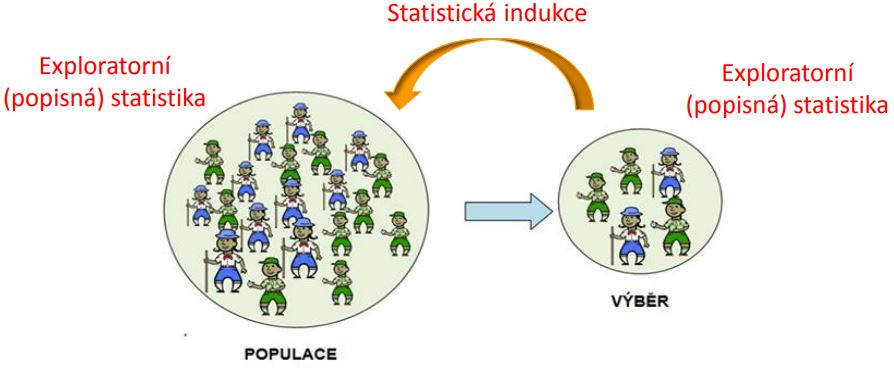
\includegraphics[width=0.6\textwidth]{assets/14_stat_ind}
\end{figure}

\textbf{Základní soubor (populace)}
\begin{itemize}
	\item Je množina všech teoreticky možných objektů (např. jedinců) v uvažované situaci = statistický soubor, který je vymezen cílem výzkumu a pro který vyvozujeme závěry výzkumného šetření.
	\item Charakterizuje se \textbf{parametrem}, což je např. výška, váha, IQ, atp.
	\item Má konečný nebo nekonečný (hypotetický) \textbf{rozsah}, který je dán N (např.: N = 150 lidí, opic, rostlin,...).
\end{itemize}
\textbf{Výběrový soubor (výběr)}
\begin{itemize}
	\item Je část populace vybrané na základě předem stanovených kritérii resp. pravidel (podmnožina základního souboru).
	\item \textbf{O náhodném výběru} uvažujeme, když splňuje dvě základní vlastnosti: pravděpodobnost zařazení do vzorku je pro všechny statistické jednotky populace nenulová a statistické jednotky jsou do vzorku vybrané nezávisle jedna od druhé.
	\item \textbf{O reprezentativním výběru} uvažujeme, když výběrový soubor dobře odráží strukturu celého zkoumaného souboru.
\end{itemize}
\textbf{Principy statistického usuzování}
\begin{enumerate}
	\item Statistické usuzování znamená zobecňování z výběrových statistik na parametry rozdělení.
	\item Abychom mohli provést statistické usuzování, musíme mít nějakou teorii, jež popisuje náhodné chování sledovaných proměnných.
	\item Existují dva typy výběrových chyb: náhodné výběrové chyby a systematické chyby. Získáním náhodného výběru zmenšujeme systematickou chybu a získáváme podklad pro odhad náhodné výběrové chyby.
	\item Výběrová rozdělení statistik jsou teoretická pravděpodobnostní rozdělení, která popisují vztah mezi výběrovou statistikou a populací.
	\item Směrodatná odchylka výběrového rozdělení statistiky (odhad parametru) se nazývá směrodatná chyba. Odhaduje náhodnou výběrovou chybu vypočítané statistiky (odhadu parametru).
	\item Jak roste velikost výběru, výběrová chyba a směrodatná chyba se zmenšují.
	\item Směrodatná chyba se používá k získání intervalového odhadu parametrů i k testování hypotéz o parametrech rozdělení.
\end{enumerate}